%!TEX root = ../../csuthesis_main.tex
\chapter{研究理论基础}

本章旨在对本研究所依赖的关键算法与基础理论进行系统阐述,为后续视觉目标跟踪与意图识别系统的实现提供理论支撑。内容包括目标检测与视觉跟踪技术的基本概念,DeepSORT 跟踪算法的原理与工作流程,以及基于速度与空间信息的意图识别模型。同时,为便于理解,还将简要介绍在本研究中承担仿真任务的 Carla 平台的相关原理。

\section{目标检测与视觉跟踪概述}

在自动驾驶系统中,环境感知是实现安全驾驶与智能决策的基础。通过计算机视觉技术识别道路上的车辆、行人、交通标志等关键对象,并对其动态状态进行连续追踪,是实现环境建模与行为预测的重要手段。目标检测与视觉跟踪作为其中的核心组成部分,直接影响着自动驾驶系统对外部环境的认知能力与决策准确性。

目标检测(Object Detection)指的是在输入图像中识别出所有存在的感兴趣目标,并准确回归其在图像中的位置(通常以边界框形式表示)以及目标类别信息。传统的目标检测算法主要依赖人工设计的特征与滑动窗口机制,代表方法如 Haar 特征与 HOG+SVM 检测器,尽管实现简单,但在复杂背景下的鲁棒性较差。近年来,随着深度学习的发展,基于卷积神经网络(CNN)的目标检测方法逐渐成为主流,显著提升了检测精度与速度。当前主流的检测模型可分为两类:一类是以 Faster R-CNN 为代表的两阶段检测器,其先生成候选区域后进行分类与回归,精度较高但速度较慢;另一类则是以 YOLO(You Only Look Once)、SSD(Single Shot MultiBox Detector)等为代表的单阶段检测器,其直接在特征图上进行回归预测,具有更高的实时性,适用于自动驾驶等对延迟要求较高的应用场景。

与目标检测不同,目标跟踪(Object Tracking)是指在已知初始检测结果的前提下,持续对目标在视频序列中的位置进行估计。根据跟踪目标的数量,通常可分为单目标跟踪(Single Object Tracking, SOT)与多目标跟踪(Multiple Object Tracking, MOT)。单目标跟踪关注于对一个特定目标进行持续跟踪,其主要挑战在于遮挡、快速运动、目标消失与再出现等;而多目标跟踪则需要同时对多个目标进行识别与数据关联,面临着更高的关联复杂性与遮挡问题。在实际的自动驾驶场景中,由于交通参与者种类多、状态变化快、相互干扰强,因此往往需在较短时间内完成高准确率的多目标跟踪任务。

视觉目标跟踪通常依赖目标检测结果作为输入,通过匹配机制完成目标的跨帧关联。跟踪算法可按是否借助外部检测结果分为两类:一类是基于检测的跟踪(Tracking-by-Detection),该类方法首先使用检测器获取每帧图像中的目标位置,然后通过轨迹预测与数据关联模块实现目标编号的一致性,是当前主流的工程实现方式;另一类是端到端的跟踪方法,直接通过时序特征建模目标的运动轨迹,适合复杂行为建模任务。前者由于易于部署与现有检测模型兼容,成为了众多自动驾驶感知系统的首选方案。

在本研究中,为提高系统的实时性与稳定性,采用了“检测—跟踪”分离式结构,即首先利用图像分析提取候选目标的边界框与状态信息,然后通过外部跟踪器(DeepSORT)进行跨帧目标关联。此结构既可以利用深度检测模型的高精度特性,又能充分结合目标的运动学特征,实现实时、连续、稳定的目标轨迹追踪。同时,单目标跟踪策略被引入,用于聚焦当前与本车存在潜在交互风险的目标,提升后续意图分析模块的准确性与实用性。

目标检测与视觉跟踪技术构成了自动驾驶系统中感知层的核心支撑,对系统的安全性、实时性与可靠性具有直接影响。在本课题中,这两项技术作为算法链条的起点,将为后续的意图识别与行为预测提供基础信息保障。


\section{DeepSORT 算法原理与流程}

在视觉目标跟踪任务中,传统的多目标跟踪(MOT)算法如 SORT(Simple Online and Realtime Tracking)因其结构简单、处理速度快,被广泛应用于实时系统中。但在复杂交通场景下,目标之间频繁遮挡、外观相似度高、轨迹交叉密集等因素,容易造成目标 ID 的切换或跟踪中断,从而降低系统的稳定性与实用性。为了解决这些问题,Wojke 等人\cite{Wojke2017DeepSORT}在2017 年提出DeepSORT(Deep Simple Online and Realtime Tracking)算法,在保持 SORT 轻量特性的基础上,引入了外观信息进行多维度数据关联,有效提升了多目标跟踪的鲁棒性和精度。

\subsection{算法结构概述}

DeepSORT 是一种基于检测驱动的在线目标跟踪算法,其整体结构由三部分组成:目标运动建模模块(卡尔曼滤波器)、数据关联模块(匈牙利算法与融合距离度量)以及外观特征提取模块。它基于SORT(Simple Online and Realtime Tracking)算法的扩展,SORT算法通过卡尔曼滤波器和匈牙利算法完成目标的状态预测与数据关联,但仅依赖于目标的运动信息进行匹配。DeepSORT则通过引入深度学习模型,利用目标的外观特征进一步增强了算法的鲁棒性和精度。算法的基本思想是:每一帧从检测器获取边界框,通过预测与匹配将其关联至已有轨迹,实现目标编号的持续与轨迹的连续。该结构兼顾精度与实时性,特别适合部署于自动驾驶等延迟敏感的系统中。

\subsection{状态预测:卡尔曼滤波器}

DeepSORT 使用卡尔曼滤波器对每个目标进行状态建模与短时位置预测。每个目标的状态向量通常定义为:
\[x = [u, v, \gamma, h, \dot{u}, \dot{v}, \dot{\gamma}, \dot{h}]^{T}\]

DeepSORT的第一步是对目标状态进行预测,而这一过程依赖于卡尔曼滤波器。卡尔曼滤波器是一种基于动态系统的状态估计方法,能够对目标的运动状态(包括位置、速度等)进行平滑和预测。在目标跟踪过程中,卡尔曼滤波器通过对上一帧目标状态的估计,预测目标在当前帧的可能位置,从而减少由于目标丢失或遮挡带来的误差。

卡尔曼滤波器的核心是基于目标的运动方程进行线性预测,结合测量值对目标的状态进行更新。在每一帧中,卡尔曼滤波器根据上一帧的目标位置与速度,预测当前帧中目标的状态,并通过目标的检测结果对预测状态进行修正。通过这种方式,卡尔曼滤波器可以保持目标的连续性,弥补检测过程中可能的丢失和误差。

\subsection{外观建模:深度特征提取}
在多目标跟踪中,目标的外观特征提取是确保算法鲁棒性和精度的关键技术之一。传统的目标跟踪算法主要依赖于目标的运动信息(如位置、速度等)进行跟踪,这种方法在处理目标遮挡、重叠或快速运动时往往效果不佳。而DeepSORT通过引入深度学习模型,特别是深度卷积神经网络(CNN),在提取目标的运动信息的同时,也结合了目标的外观特征,大大增强了算法在复杂场景中的跟踪精度。

DeepSORT的外观建模部分通过使用卷积神经网络(CNN)来提取目标的视觉特征。这些特征通常包含了目标的颜色、形状、纹理等信息,有助于区分不同目标,特别是在多目标重叠或目标短时间遮挡的情况下,外观特征能够有效解决身份混淆问题。CNN通过对目标边界框区域进行裁剪,并将裁剪后的图像输入网络,从中提取出固定维度的特征向量。这个向量就是目标的外观特征,表示了目标的独特视觉信息。

通过外观特征的提取,DeepSORT能够在跟踪过程中通过比对目标在不同帧中的特征向量,来识别和区分不同目标。这一方法极大地提升了算法在复杂动态环境中的表现,尤其在目标交叉和长时间遮挡的情况下,外观特征提供了目标身份的持续确认。

然而,外观特征提取并非没有挑战。在多目标跟踪中,目标的外观特征可能会受到光照、角度变化或其他环境因素的影响,导致目标的视觉特征发生变化。因此,如何保持特征的一致性,并在变化条件下进行有效匹配,是DeepSORT面临的一个重要问题。针对这一问题,未来的研究可以通过改进深度网络结构或结合其他特征提取方法,进一步提升外观建模的鲁棒性。

总结而言,DeepSORT通过引入深度学习的外观特征提取机制,使得算法不仅仅依赖于目标的运动信息,还能够通过视觉特征有效区分目标,提高了跟踪精度和鲁棒性。这一技术在动态复杂场景中的应用具有重要的实际意义,尤其适用于自动驾驶、智能监控等需要精确多目标跟踪的领域。

\subsection{匹配决策:融合距离与匈牙利算法}
在多目标跟踪任务中,目标的匹配决策是确保跟踪精度和一致性的关键步骤。DeepSORT算法通过结合目标的运动信息和外观特征来进行目标的匹配,从而避免了仅依赖运动信息导致的身份混淆和丢失问题。匹配决策的核心在于通过计算目标之间的相似度,并采用优化算法(如匈牙利算法)进行最优匹配。

DeepSORT通过融合两种信息来决定目标的匹配:一种是基于目标位置的欧氏距离,另一种是基于目标外观特征的相似度。通过这两种信息的结合,DeepSORT能够更精确地判断当前帧中的检测框是否与上一帧中的目标相对应。具体而言,欧氏距离用于衡量目标在空间中的位置变化,而外观特征的相似度则反映了目标在视觉空间中的一致性。

\textbf{欧氏距离:}在多目标跟踪中,目标的位置变化通常表现为目标的运动。欧氏距离是衡量目标在图像空间中位置变化的常用度量,它计算目标在两帧图像中的位置差异。目标间的运动距离越小,说明它们之间的关系越紧密,因此位置上的距离差异成为目标匹配的重要依据。

\textbf{外观特征的相似度:}为了进一步提高匹配的精度,DeepSORT利用目标的外观特征来进行匹配。外观特征是通过深度卷积神经网络提取的,包含了目标的颜色、纹理、形状等信息。通过计算当前帧目标的外观特征与上一帧目标特征的相似度,DeepSORT可以判断两个目标是否为同一目标,即使它们的位置发生了变化。

在DeepSORT中,目标的匹配决策是通过计算每一对目标的匹配代价来完成的。代价矩阵是由目标之间的欧氏距离和外观特征相似度组成的,这两种信息被结合成一个综合的匹配代价。在这个代价矩阵中,每一对目标之间的代价反映了它们之间的匹配难度,代价越低,匹配越精确。

为了从代价矩阵中选出最优匹配,DeepSORT使用了匈牙利算法。匈牙利算法是一种解决二分图匹配问题的经典算法,能够在代价矩阵中找到最小匹配代价,从而实现目标的最优匹配。通过匈牙利算法,DeepSORT能够在当前帧和上一帧之间找到最佳匹配关系,确保目标的身份一致性,并且最大限度地减少了匹配错误。

在实际应用中,匈牙利算法通过最优化匹配代价的方式,解决了数据关联中目标匹配的问题。它通过将目标检测框与已知目标进行比较,寻找最佳的匹配对。在复杂的动态场景中,匈牙利算法能够在目标之间建立准确的匹配关系,从而减少了目标丢失和身份混淆的情况。

\subsection{算法执行流程}

DeepSORT的处理流程包括多个步骤,以下是每一帧图像的执行流程:

\textbf{接收当前帧图像和检测器输出(边界框): }在每一帧中,DeepSORT首先接收当前帧图像以及通过目标检测算法(如YOLO、Faster R-CNN等)输出的边界框。这些边界框包含了每个目标的位置、尺寸以及检测的置信度。

\textbf{对当前所有轨迹通过卡尔曼滤波器进行状态预测: }对于所有已知的目标轨迹,DeepSORT使用卡尔曼滤波器来预测它们的状态(即位置和速度)。卡尔曼滤波器基于目标上一帧的位置和速度信息,对目标进行平滑并预测其在当前帧的位置。这一步骤有助于弥补由于目标丢失或遮挡导致的检测信息缺失。

\textbf{对当前检测框提取外观特征向量: }DeepSORT使用预训练的深度卷积神经网络(CNN)提取每个目标的外观特征。这些外观特征可以描述目标的颜色、纹理、形状等视觉信息。通过这些特征,DeepSORT能够有效地区分不同目标,即使在目标相互遮挡或位置变化较大的情况下,仍能准确识别和跟踪目标。

\textbf{构建融合距离矩阵并输入匈牙利算法匹配轨迹与检测: }DeepSORT根据目标的运动信息和外观特征构建融合距离矩阵。该矩阵计算每个检测框与当前跟踪轨迹之间的匹配度,既包括基于位置的欧氏距离,也包括基于外观特征的相似度。然后,使用匈牙利算法对目标进行最优化匹配,确保每个目标在当前帧和上一帧之间能够精确对应。

\textbf{对匹配成功的轨迹执行更新,未匹配项处理为新轨迹或丢失轨迹: }对于匹配成功的目标,DeepSORT将更新其位置、速度等信息。对于未匹配的目标,DeepSORT根据设定的规则决定是将其视为新轨迹(即新检测到的目标),还是将其视为丢失轨迹。丢失轨迹会根据卡尔曼滤波器的预测持续保持其状态,直到目标重新出现或超出设定的丢失阈值。

\textbf{输出每个有效轨迹的编号与位置: }最终,DeepSORT会输出每个有效的目标轨迹,包括目标的编号、位置等信息。每个目标在整个跟踪过程中都有一个唯一的ID,确保目标的身份在所有帧中保持一致。

该流程在每一帧图像中独立运行,并且能够实时更新目标的状态,因此具有良好的在线处理能力,特别适合低延迟的自动驾驶系统、智能监控等实时应用场景。通过这一系列步骤,DeepSORT能够实现多目标的精准跟踪,并在复杂场景下保持高效的实时性。
\begin{figure}[H]
    \centering
    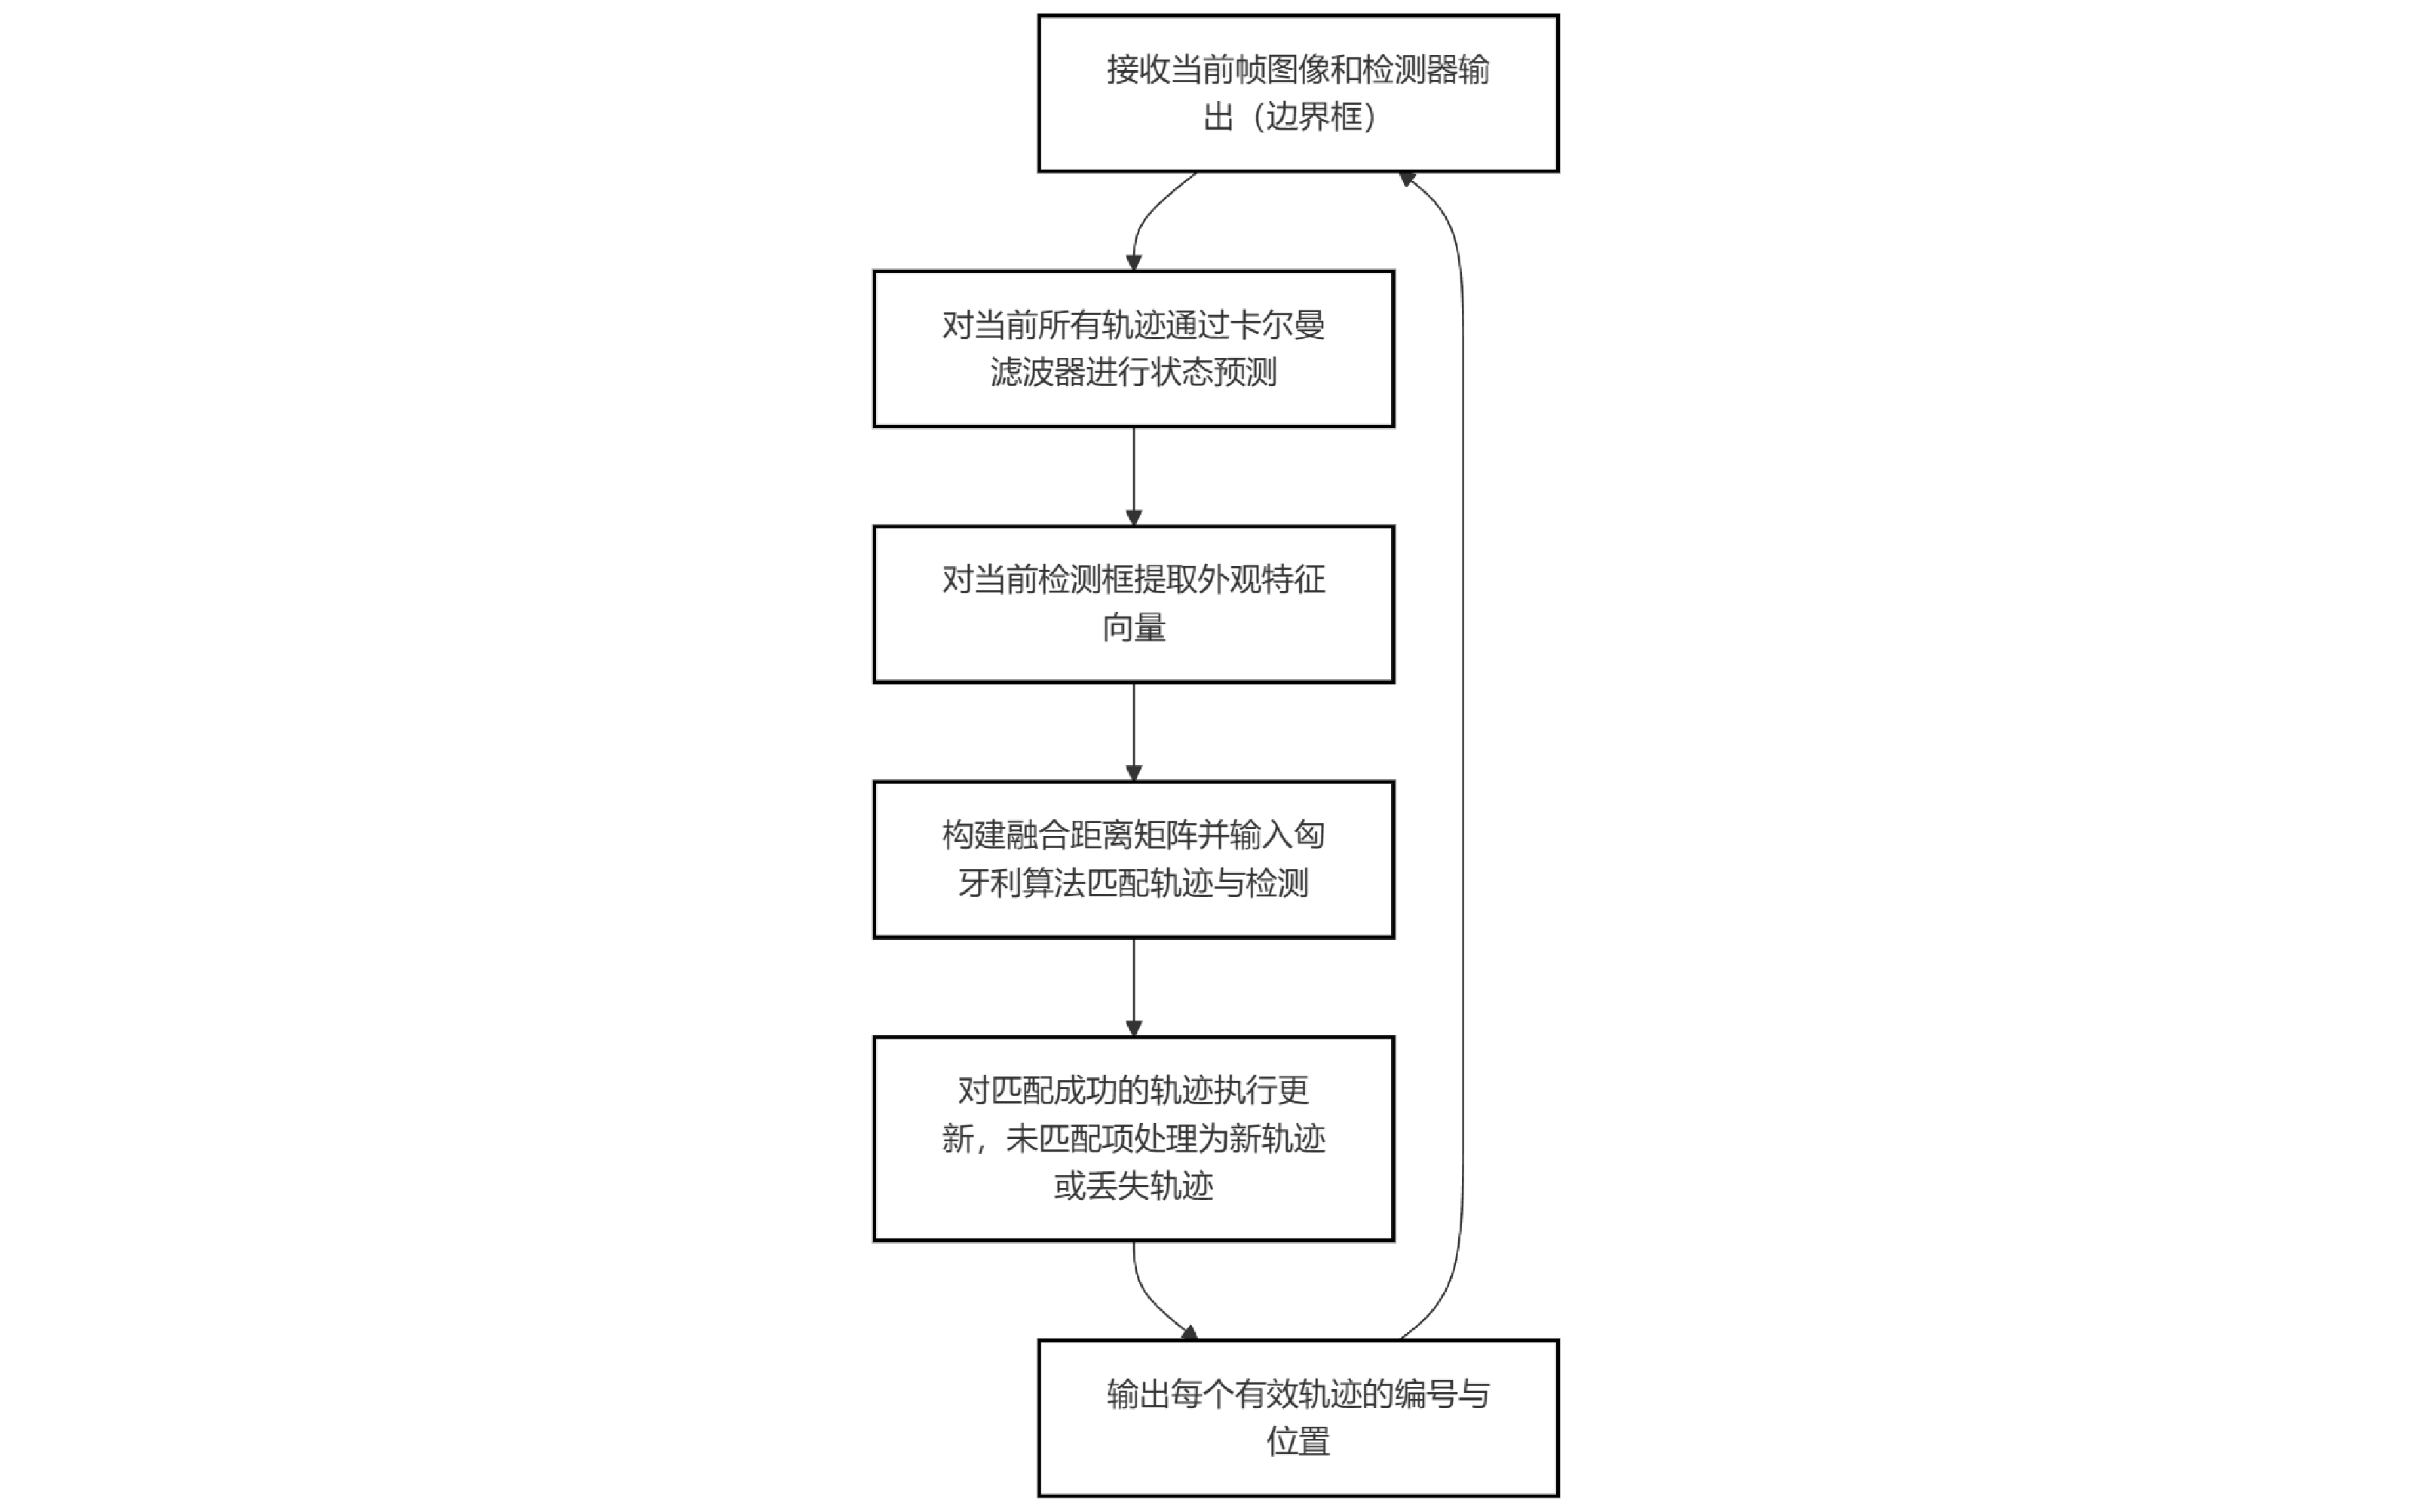
\includegraphics[width=0.8\textwidth]{images/图2 DeepSORT算法执行流程.pdf}  % 引用转换后的 PDF 文件
    \caption{DeepSORT算法执行流程}
    \label{fig:example_image}  % 可用于引用此图片
\end{figure}

\section{行为意图识别的物理建模方法}

在自动驾驶系统中,车辆仅具备对环境中物体的“检测”与“跟踪”能力是远远不够的。为了实现更高级别的决策控制与路径规划,系统还需对周围交通参与者的行为意图进行识别,即判断其未来可能的运动趋势与与本车的相对风险关系。行为意图分析不仅关系到驾驶安全,也直接影响车辆的行为生成策略,因此被认为是连接感知与决策的关键桥梁。在本课题中,针对城市交通环境下的典型车辆交互场景,设计了一套基于物理状态信息的行为意图判别方法,构建了一套可嵌入至视觉跟踪系统中的轻量级意图分析模块。

\subsection{意图识别的物理基础}

本研究所采用的行为意图识别方法,基于目标的相对位置变化与瞬时速度信息,构建了一种近似物理建模的分析机制。设定某一时刻跟踪目标的二维图像平面投影中心($x_t$,$y_t$),上一时刻为($x_{t-1}$,$y_{t-1}$),自车屏幕参考点位置为($x_c$,$y_c$)。则目标相对位置变化量可定义为:
\[\Delta d = \|(x_t, y_t) - (x_c, y_c)\| - \|(x_{t - 1}, y_{t - 1}) - (x_c, y_c)\|\]

其中,$\left| \cdot \right|$表示欧几里得距离。该值用于衡量目标与自车的相对距离变化趋势。结合目标的瞬时速度$v_t$,可初步判断其运动意图。

此外,为增强分析的动态敏感性,引入了前后帧距离差分值$\Delta d$与速度 $v_t$的联合判断阈值规则。通过组合判断目标是否正在靠近本车、远离、停留或加速穿越等,从而实现意图的粗分类。这种方法不依赖于轨迹预测或时序模型,具有实现简单、计算开销小、适用于实时系统等优点。

\subsection{判别规则设计与分类逻辑}

在本研究系统中,结合实验场景和工程实现,设计了以下几种典型的行为状态分类逻辑:

\textbf{目标靠近中:}当$\Delta d < -\delta_{\mathrm{d}}$且$v_t>v_{\text{min}}$时,表明目标正在快速靠近自车;

\textbf{目标远离中:}当$\Delta d > -\delta_{\mathrm{d}}$时,目标正在逐渐离开;

\textbf{危险靠近:}若当前距离低于设定阈值$d_{\text{critical}}$且速度超过$v_{\text{danger}}$时,则标记为潜在危险行为;

\textbf{目标稳定:}若目标距离变化缓慢或速度较低,判断为意图不明或保持状态;

\textbf{目标初始化中:}用于系统首次观测目标,未形成完整判断所处状态。

上述分类逻辑采用了硬阈值判定策略,其参数$\delta_{\mathrm{d}}$、$v_{\text{min}}$、$v_{\text{danger}}$、$d_{\text{critical}}$均可根据场景密度或车辆速度进行调节。在实验中,采用经验法则设定$\delta_{\mathrm{d}}$=5、$v_{\text{min}}$=1.5m/s、$v_{\text{danger}}$=3.0m/s、$d_{\text{critical}}$=150(像素),实现了较高的判别正确率。

\subsection{与视觉跟踪系统的集成实现}

本意图分析模块在实现上嵌入至单目标跟踪模块之后,通过对被选中目标的时序状态进行分析,输出当前帧的意图状态描述文本,并在图像上实时展示。此外,模块设计了状态缓存机制,保证判断结果具备一定的时间一致性,避免因短时检测误差导致意图抖动。

在 Carla 仿真平台的 Town10 与 Town01 场景中,该模块成功实现了对前方车辆是否构成“威胁靠近”或“远离离散”的视觉提示,提升了系统的交互解释性与安全响应能力,为后续的路径规划与驾驶行为生成提供了语义输入支持。

\section{小结}
本章围绕“视觉目标跟踪与行为意图识别”在自动驾驶系统中的核心作用,系统阐述了本课题研究所依赖的相关理论与关键技术。首先,针对当前智能驾驶车辆在动态环境中感知能力的提升需求,简要回顾了目标检测与视觉跟踪的发展历程,分析了从基于运动建模的传统跟踪方法,到融合检测器输出与深度特征的现代方法的技术演进。通过对视觉感知链条的梳理,明确了视觉跟踪在动态交通场景中对目标连续性、身份保持与行为识别的不可替代作用。

其次,论文重点解析了本研究中所采用的 DeepSORT 算法的核心原理与完整处理流程。该算法在保持传统 SORT 算法速度优势的同时,引入外观特征建模机制,有效缓解了目标遮挡、遮蔽后 re-identification(再识别)失败等问题。论文对 DeepSORT 中的卡尔曼滤波器状态建模、ReID 特征提取网络、马氏距离与余弦距离的融合度量机制,以及轨迹匹配与更新策略进行了逐一解析。同时也说明了该算法在本系统中的实际应用方式,包括如何结合检测结果实现在线目标轨迹更新,并输出稳定、可控的目标标识编号,为后续高层语义分析打下基础。

在第三部分中,本章还深入探讨了行为意图识别的物理建模方法。相较于基于深度学习的预测模型或时序模型,本研究采用了更加轻量、高效、适用于实时场景的基于位置与速度信息的规则建模策略。该方法利用相对距离变化与目标运动速度联合构建了一个多条件的判别机制,从而可实现“靠近”、“远离”、“危险接近”等典型语义意图的有效识别。该模块在实现层面被集成至目标跟踪逻辑之后,通过连续帧数据的物理量计算,结合阈值策略实现了对动态交互行为的解释与预警。同时,为增强系统交互性与直观表达,本研究还设计了对应的可视化机制,将判别结果实时叠加至目标标注框上方,提升了系统对复杂交通行为的响应能力与解释能力。

综合来看,本章从理论出发,系统梳理了本课题中所涉及的视觉感知、目标跟踪与行为理解的关键环节,为后续系统功能的整体实现提供了坚实的技术基础。下一章将在本章理论基础之上,详细展开系统总体架构的设计思路,包括 Carla 仿真平台的部署配置、自动驾驶控制主模块的构建方式、以及整体工程开发环境的搭建方案,从工程角度推进本研究方案的具体实现。



\begin{tabular}{l l}
%  \verb|\songti| & {\songti 宋体} \\
%  \verb|\heiti| & {\heiti 黑体} \\
%   \verb|\kaiti| & {\kaiti 楷体}
\end{tabular}
